
\section{态射为\trClosedEmbedding{}的一个判别法}

我们将反复使用一个判定\trMorphism{}何时为\trClosedEmbedding{}的判别法，它并非\trCurve{}所独有。在陈述它之前，我们先回忆一些关于\trClosedEmbedding{}的事实。设 $\pi\colon X\to Y$ 是一个\trClosedEmbedding。那么 $\pi$ 是\trProjective{}的，并且在点上单射。仅凭这些还不足以保证它是\trClosedEmbedding{}——\trCusp{}的\trNormalization{}这个例子（图~\ref{fig:cusp-normalization}）便表明了这一点。另一个例子是下面这道练习。

\textbf{19.1.A.（练习：\trFrobenius；参看 \S8.3.Q）}\quad 证明：由 $x\mapsto x^{p}$ 给出的 $\pi\colon\mathbb{A}^1_{\mathbb{F}_p}\to\mathbb{A}^1_{\mathbb{F}_p}$ 在点上双射，并且在\trClosedPoint{}上诱导\trResidueField{}的同构，然而它并不是\trClosedEmbedding。

为了使一个\trMorphism{} $\pi$ 是\trClosedEmbedding，你所需要的附加信息是：切映射在一切\trClosedPoint{}处都是单射。

\textbf{19.1.B.（练习）}\quad 证明（直接证明，不要援引\mbox{定理~19.1.1}）：在上文描述的两个例子（\trCusp{}的\trNormalization{}与\trFrobenius{}态射）中，切映射在一切\trClosedPoint{}处都\emph{不}单射。

\textbf{19.1.1.\ \trhTheorem。}\ ——\ \emph{设 $k=\overline{k}$，而 $\pi\colon X\to Y$ 是有限型 $k$-\trScheme{}之间的一个\trProjective\trMorphism，它在\trClosedPoint{}上单射，并且在\trClosedPoint{}处的\trTangentVector{}上单射。那么 $\pi$ 是一个\trClosedEmbedding。}

逆命题是显然的，所以你应当把这个结果当作「当且仅当」来用。

（注记：对于代数闭域上的有限型概形这一情形，「在\trClosedPoint{}处的\trTangentVector{}上单射」等价于「\trUnramified」；见\mbox{练习~21.7.E}。我们将在 \S21.7 中定义\trUnramified。）

例子 $\Spec\mathbb{C}\to\Spec\mathbb{R}$ 表明：在\mbox{定理~19.1.1} 中我们确实需要「$k$ 是\trAlgClosed{}的」这条假设。对\trAlgClosedField{}过敏的读者也请留心，因为我们将用它来证明关于 $k$ 上\trCurve{}的一些结果，其中 $k$ \emph{未必}是\trAlgClosed{}的（另见\mbox{练习~10.2.K} 与\mbox{练习~19.1.F}）。

我们还需要「该\trMorphism{}是\trProjective{}的」这条假设，图~\ref{fig:projectivity-node-example} 的例子表明了这一点。这个例子是\trNode{}的\trNormalization{}，只是我们把\trNode{}的诸原像之一擦去了。我们把 $\mathbb{A}^1$ 映入平面，使得它的像是一条带一个\trNode{}的\trCurve。然后我们考虑丢弃\trNode{}的一个原像之后所得的\trMorphism。此时这个\trMorphism{}在点上单射，并且在\trTangentVector{}上也单射，但它不是\trClosedEmbedding{}。（在\trDifferentialGeometry{}的世界里，它之所以算不得嵌入，是因为这个映射不给出到其像上的\trHomeomorphism。）

\begin{figure}[htbp]
\centering
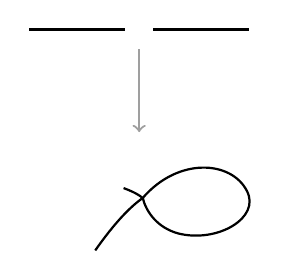
\begin{tikzpicture}[scale=0.9,line width=0.8pt]
  \draw[line width=1.2pt] (-1.55,2.40) -- (-0.20,2.40);
  \draw[line width=1.2pt] (0.20,2.40) -- (1.55,2.40);
  \draw[gray!75,->] (0,2.12) -- (0,0.95);
  \draw (0.05,0.02) .. controls (0.55,0.60) and (1.30,0.55) .. (1.52,0.12)
        .. controls (1.72,-0.26) and (1.10,-0.62) .. (0.55,-0.48)
        .. controls (0.26,-0.40) and (0.10,-0.18) .. (0.05,0.02);
  \draw (-0.22,0.16) .. controls (-0.06,0.10) and (0.00,0.06) .. (0.05,0.02)
        .. controls (-0.12,-0.10) and (-0.34,-0.32) .. (-0.62,-0.72);
\end{tikzpicture}
\caption{（图~\ref{fig:normalization-nodal-cubic} 的变体）\mbox{定理~19.1.1} 中的\trProjective{}性假设不能去掉。（依原书手绘图重绘。）}\label{fig:projectivity-node-example}
\end{figure}

\mbox{定理~19.1.1} 看上去根本上是关于\trVariety{}的一个陈述，但其实并不是。我们将把它化归为下面的结果。

\textbf{19.1.2.\ \trhTheorem。}\ ——\ \emph{设 $\pi\colon X\to Y$ 是\trNoetherian{}\trScheme{}之间的一个\trFinite\trMorphism，它在 $Y$ 的每一点处的次数（\S14.3.4）为 $0$ 或 $1$。那么 $\pi$ 是一个\trClosedEmbedding。}

\textbf{19.1.C.（练习）}\quad 设 $\pi\colon X\to Y$ 是一个\trFinite\trMorphism，它在 $Y$ 的每一点处的次数为 $0$ 或 $1$。证明：$\pi$ 在点上单射（容易）。若 $p\in X$ 是任一点，证明 $\pi$ 诱导\trResidueField{}的同构 $\kappa(\pi(p))\overset{\sim}{\longrightarrow}\kappa(p)$。证明 $\pi$ 诱导\trTangentSpace{}之间的一个单射。于是，\mbox{定理~19.1.1} 的几条关键假设便都隐含在\mbox{定理~19.1.2} 的假设之中了。

\textbf{19.1.3.}\ \emph{\mbox{定理~19.1.1} 到\mbox{定理~19.1.2} 的化归。}\quad 「是\trClosedEmbedding」这一性质在靶上是局部的，故我们不妨假设 $Y$ 是\trAffine{}的，比如说 $\Spec B$。

接下来我断言：$\pi$ 具有\trFinite\trFiber——而不只是在\trClosedPoint{}之上\trFiber{}有限：\trProjective\trMorphism{}的纤维维数是\trUpperSemicontinuous{}的（\mbox{练习~18.1.B}，或\mbox{定理~12.4.3(b)}），于是纤维维数至少为 $1$ 的那个\trLocus{}是一个\trClosedSubset，从而若它非空，就必然含有 $Y$ 的一个\trClosedPoint。于是，任一点之上的\trFiber{}都是该点之上的维数 $0$ 的有限型\trScheme，因而是个\trFinite{}集。

于是 $\pi$ 是一个带\trFinite\trFiber{}的\trProjective\trMorphism，从而由\mbox{定理~18.1.6} 是\trFinite{}的。

\textbf{19.1.D.（练习）}\quad 证明：$\pi$ 的次数在 $Y$ 的一切\trClosedPoint{}处都至多为 $1$。（提示一：这里你将用到「在\trTangentVector{}上单射」这条假设。提示二：到 $\Spec\overline{k}$ 的\trFinite\trMorphism{}都有哪些？）

但\trFinite\trMorphism{}的次数是\trUpperSemicontinuous{}的（\S14.3.4），故在一切点处都至多为 $1$（你看出这是为什么了吗？）。这样我们便证明了：\mbox{定理~19.1.1} 可以由\mbox{定理~19.1.2} 推出。

\textbf{19.1.4.}\ \emph{\mbox{定理~19.1.2} 的证明。}\quad 这个问题在 $Y$ 上是局部的，故我们不妨假设 $Y$ 是\trAffine{}的，比如说 $Y=\Spec B$。于是 $X$ 也是\trAffine{}的，比如说 $\Spec A$，而 $\pi$ 对应于一个\trRingMorphism{} $B\to A$。我们想证明这是一个环的满射，或者（等价地）$B$-\trModule{}的满射。令 $K$ 是这个 $B$-\trModule{}态射的\trCokernel：
\begin{equation*}\tag{19.1.4.1}\label{eq:criterion-cokernel-sequence}
B\longrightarrow A\longrightarrow K\longrightarrow 0.
\end{equation*}
我们想证明 $K=0$。只须证明：对 $B$ 的任意\trMaximalIdeal{} $\mathfrak{n}$ 都有 $K_{\mathfrak{n}}=0$。（你还记得这是为什么吗？）把 \eqref{eq:criterion-cokernel-sequence} 在 $\mathfrak{n}$ 处局部化，便得到正合列
\[
B_{\mathfrak{n}}\longrightarrow A_{\mathfrak{n}}\longrightarrow K_{\mathfrak{n}}\longrightarrow 0.
\]
施加右正合函子 $\otimes_{B_{\mathfrak{n}}}(B_{\mathfrak{n}}/\mathfrak{n}B_{\mathfrak{n}})$，便得
\begin{equation*}\tag{19.1.4.2}\label{eq:criterion-tensor-cokernel-sequence}
B_{\mathfrak{n}}/\mathfrak{n}B_{\mathfrak{n}}\overset{\alpha}{\longrightarrow}A_{\mathfrak{n}}/\mathfrak{n}A_{\mathfrak{n}}\longrightarrow K_{\mathfrak{n}}/\mathfrak{n}K_{\mathfrak{n}}\longrightarrow 0.
\end{equation*}
现在 $\Spec A_{\mathfrak{n}}/\mathfrak{n}A_{\mathfrak{n}}$ 是 $[\mathfrak{n}]\in\Spec B$ 的\trSchemeTheoreticPreimage，故由假设，它要么是空的，要么映射 $\alpha$ 是同构（在这一情形，我们将会看到 $\alpha$ 原来就是剩余域的映射）。在前一情形，$A_{\mathfrak{n}}/\mathfrak{n}A_{\mathfrak{n}}=0$，从而 $K_{\mathfrak{n}}/\mathfrak{n}K_{\mathfrak{n}}=0$；在后一情形，同样有 $K_{\mathfrak{n}}/\mathfrak{n}K_{\mathfrak{n}}=0$。施加\trNakayama{}引理~8.2.9（注意 $A$ 是有限生成的 $B$-\trModule，因而 $K$ 亦然，进而 $K_{\mathfrak{n}}$ 是有限生成的 $B_{\mathfrak{n}}$-\trModule），便得 $K_{\mathfrak{n}}=0$，正如所求。\hfill$\square$

\mbox{练习~10.2.K} 可以用来把\mbox{定理~19.1.1} 的效力延伸到一般的域 $k$——不必是\trAlgClosed{}的域。下面的练习就是一个例子，示范怎么做。

\textbf{19.1.E.（练习）}\quad 用\mbox{定理~19.1.1} 证明：从 $\mathbb{P}^n_k$ 出发、相应于完全线性系 $|\OO_{\mathbb{P}^n_k}(d)|$ 的第 $d$ 次\trVeroneseEmbedding{}是一个\trClosedEmbedding。对从 $\mathbb{P}^m_k\times_{\Spec k}\mathbb{P}^n_k$ 出发的\trSegre{}嵌入做同样的事。（这只是为了练习使用这个判别法。它比我们先前的结果要弱；这两条陈述我们先前都已在任意基环上验证过——分别在\mbox{注记~9.3.8} 与 \S10.6——而现在我们只在域上验证。不过，请参看下面的\mbox{练习~19.1.F}。）

\textbf{19.1.F.（较不重要的练习）}\quad 用本节的想法证明：从 $\mathbb{P}^n_{\mathbb{Z}}$（在整数环上！）出发的第 $d$ 次\trVeroneseEmbedding{}是一个\trClosedEmbedding。（再说一次，这件事我们以前做过。这道练习只是要表明：这些方法可以轻松推广，在更一般的情形同样奏效。）
